\documentclass[tikz,border=10pt]{standalone}
\usepackage{pgfplots}
\pgfplotsset{compat=newest}
% \pgfplotsset{compat=1.18}
\usepackage[american]{circuitikz}
\usepackage{cmbright}
\usetikzlibrary{fit}

\definecolor{myred}{RGB}{170,0,0}
\definecolor{myblue}{RGB}{0,0,220}
\definecolor{mygreen}{RGB}{0,150,0}
\definecolor{myorange}{RGB}{255,127,0}
\definecolor{mybrown}{RGB}{150,75,0}

\ctikzset{bipoles/resistor/height=0.2}
\ctikzset{bipoles/resistor/width=0.5}
\ctikzset{bipoles/capacitor/height=0.4}
\ctikzset{bipoles/capacitor/width=0.15}


\begin{document}
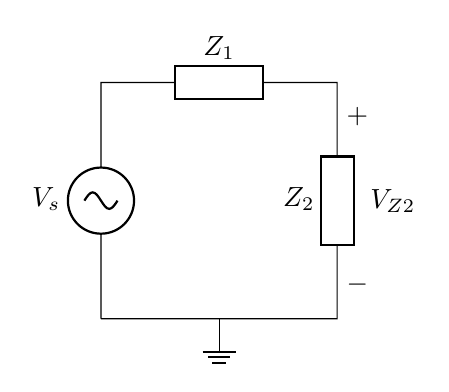
\begin{tikzpicture}
\begin{scope}
    % Nodes
    \draw (0,0) to[sV, l=$V_s$] (0,3) 
              to[generic, l=$Z_1$] (3,3)
              to[generic, l_=$Z_2$, v^>=$V_{Z2}$] (3,0)
              -- (0,0);
    \draw (1.5, 0) node[ground]{};
\end{scope}
\end{tikzpicture}

\end{document}